见 Rudin 《实分析与复分析》

\section{解析函数基本性质}

A \textbf{region} is  nonempty connected open subset of $\mathbb{C}$. Each open set $\Omega$ in the plane is union of discs. For $z_0\in \Omega$ if $\lim_{ z \to z_0 }\frac{f(z)-f(z_0)}{z-z_0}$ exists then denote it $f'(z_0)$. If $f'(z_0)$ exists $\forall z_0\in \Omega$, say $f\in H(\Omega)$. $H(\Omega)$ is the class of all holomorphic functions in $\Omega$, which is a ring. If $f$ is representable by power series in $\Omega$, then $f\in H (\Omega)$ and $f'$ is also representable. Check the convergence by evaluate
\[
\frac{\overbrace{ f(z) }^{ \sum c_nz^{n} }-f(w)}{z-w}-\underbrace{ g(w) }_{  \sum nc_nz^{n-1} }=\sum_{n=1}^{\infty} c_n\underbrace{ \left[ \frac{z^{n}-w^{n}}{z-w}-nw^{n-1}U \right] }_{ =(z-w)\sum_{k=1}^{n-1} kw^{k-1}z^{n-k-1} }
\]
Fix $w\in D(a;r)$, and choose $\rho$ s.t.$\lvert w \rvert<\rho<r$, where $r^{-1}=\limsup_{ n \to \infty }\lvert c_n \rvert ^{\frac{1}{n}}$. For $n\geq2$, if $\lvert z \rvert<\rho$ then
\[
\left\lvert  \sum_{k=1}^{n-1} kw^{k-1}z^{n-k-1}  \right\rvert \leq \frac{n(n-1)}{2}\rho^{n-2}
\]
Then
\[
\left\lvert  \frac{f(z)-f(w)}{z-w}-g(w)  \right\rvert \leq \lvert z-w \rvert \underbrace{ \sum_{n=2}^{\infty} n^2\lvert c_n \rvert \rho^{n-2} }_{ \text{converges} }\to0\qquad \text{as }z\to w
\]
An general result is for complex (finite) measure on a measurable space $X$, $\varphi$ is a plex measurable function on $X$, $\Omega$ is an open set in the plane which does not intersect $\varphi(X)$ and
\[
f(z)=\int_{X}^{} \frac{d\mu(\zeta)}{\varphi(\zeta)-z}\qquad z\in \Omega
\]
Then $f$ is \textbf{representable by power series} in $\Omega$.

The proof is from the fact that for $z\in D(a;r)\subset \Omega$, every $\zeta\in X$,
\[
\sum_{n=0}^{\infty} \frac{(z-a)^{n}}{(\varphi(\zeta)-a)^{n+1}}=\frac{1}{\varphi(\zeta)-z}
\]
Converges uniformly on $X$. Then
\[
f(z)= \int_{X}^{} \frac{d\mu(\zeta)}{\varphi(\zeta)-z}=\int_{X}^{}\sum_{n=0}^{\infty} \frac{(z-a)^{n}}{(\varphi(\zeta)-a)^{n+1}}d\mu(\zeta)=\sum_{n=0}^{\infty}\underbrace{  \left[ \int_{X}^{} \frac{d\mu(\zeta)}{(\varphi(\zeta)-a)^{n+1}}  \right] }_{ \coloneqq c_n }(z-a)^{n}
\]
Suppose $\gamma:[\alpha,\beta]\to\gamma^{*}$ a path, $f$ a continuous function defined on $\gamma^{*}$ (the range of $\gamma$), then
\[
\int_{\gamma}^{} f(z) \, dz =\int_{\alpha}^{\beta} f(\gamma(t))\gamma'(t) \, dt 
\]
$\gamma$ is unique under continuously differentaible one-to-one mapping.

Let $\gamma$ be a closed path, $\Omega$ the complement of $\gamma^{*}$, and define
\[
\mathrm{Ind}_{\gamma}(z)=\frac{1}{2\pi i}\int_{\gamma}^{} \frac{d\zeta}{\zeta-z} \qquad z\in \Omega
\]
Then $\operatorname{Ind}_\gamma$ is an integer-valued function on $\Omega$ which is constant in each component of $\Omega$ and which is 0 in the unbounded component of $\Omega$.

\begin{note}
We call $\mathrm{Ind}_{\gamma}$ the index of $z$ w.r.t. $\gamma$, which is "the number of times $\gamma$ winds around $z$".
\end{note}
\begin{figure}[H]
\centering
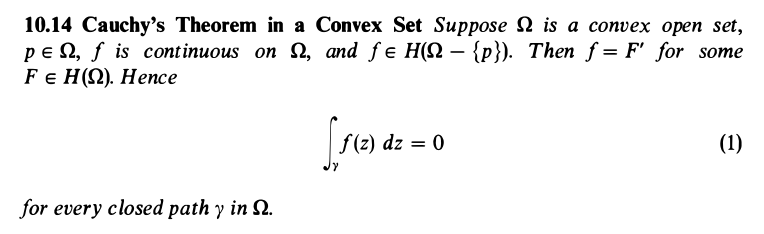
\includegraphics[width=\textwidth]{复分析脉络-2025040416.png}
% \caption{}
\label{}
\end{figure}
\begin{figure}[H]
\centering
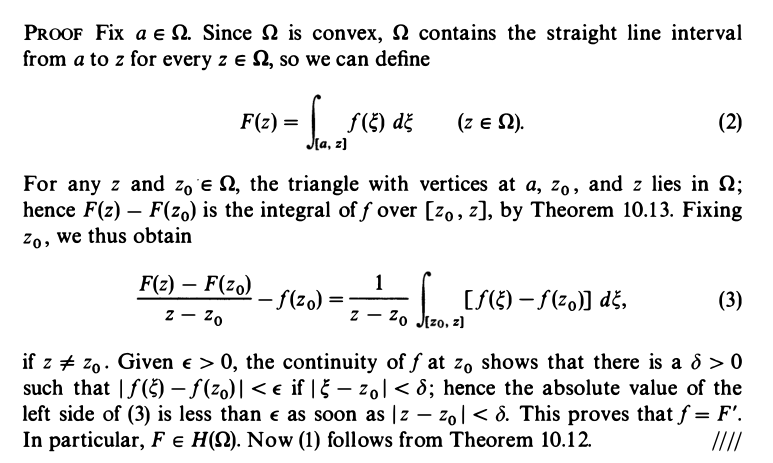
\includegraphics[width=\textwidth]{2-复分析脉络-2025040416.png}
% \caption{}
\label{}
\end{figure}
\begin{figure}[H]
\centering
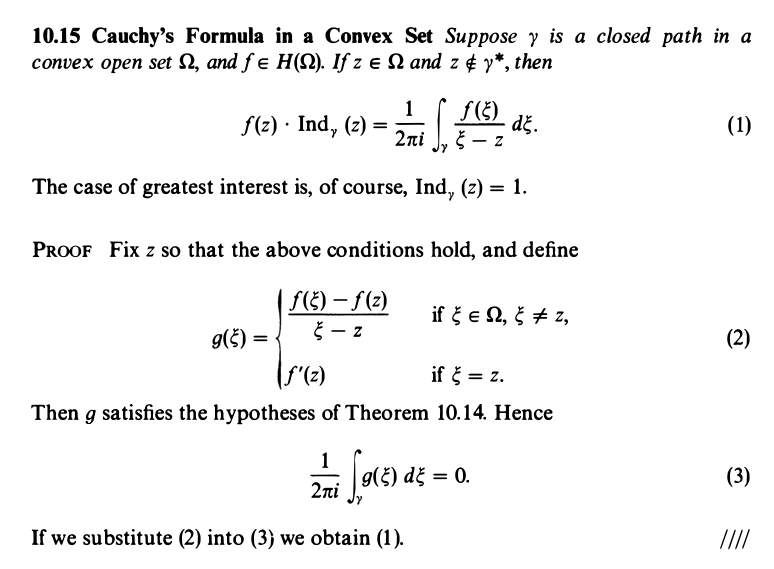
\includegraphics[width=\textwidth]{1-复分析脉络-2025040416.png}
% \caption{}
\label{}
\end{figure}

The easy consequence of the above theorem is the representability of holomorphic functions by power series.

The Cauchy theorem has a useful convers:
\begin{figure}[H]
\centering
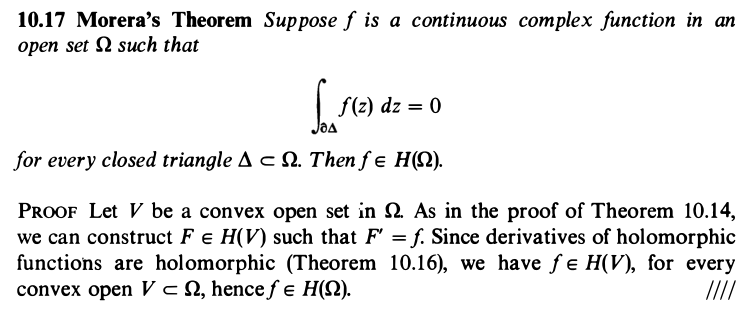
\includegraphics[width=\textwidth]{3-复分析脉络-2025040416.png}
% \caption{}
\label{}
\end{figure}
Next we consider the power series representation of holomorphic functions. Suppose $\Omega$ a region, $f\in H(\Omega)$ and $Z(f)=\{ a\in \Omega:f(a)=0 \}$. Then either $Z(f)=\Omega$ or $Z(f)$ has no limit point in $\Omega$. In the later case $\exists a\mapsto m=m(a)$ such that $f(z)=(z-a)^{m}g(z)$ for $z\in \Omega$, where $g\in H(\Omega)$ and $g(a)\neq0$. Furthermore, $Z(f)$ is at most countable.

Analogous results hold of course ofor the set of $\alpha$ -points of $f$, i.e. the zero set of $f-\alpha$.

\begin{figure}[H]
\centering
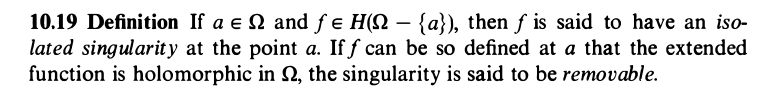
\includegraphics[width=\textwidth]{4-复分析脉络-2025040416.png}
% \caption{}
\label{}
\end{figure}

\begin{figure}[H]
\centering
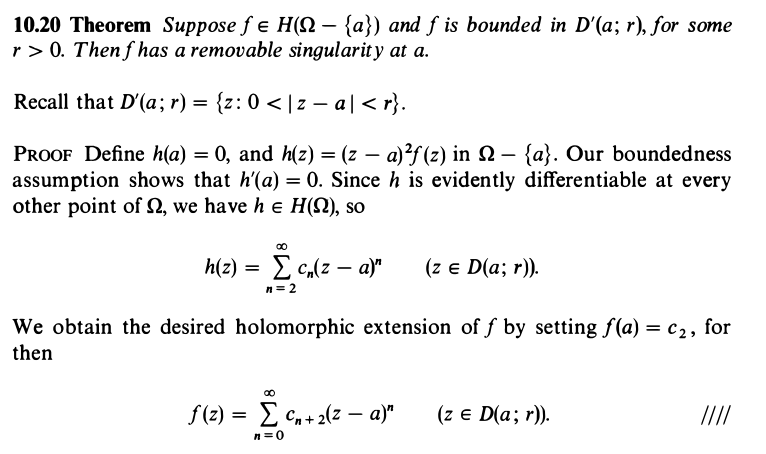
\includegraphics[width=\textwidth]{5-复分析脉络-2025040416.png}
% \caption{}
\label{}
\end{figure}

\begin{figure}[H]
\centering
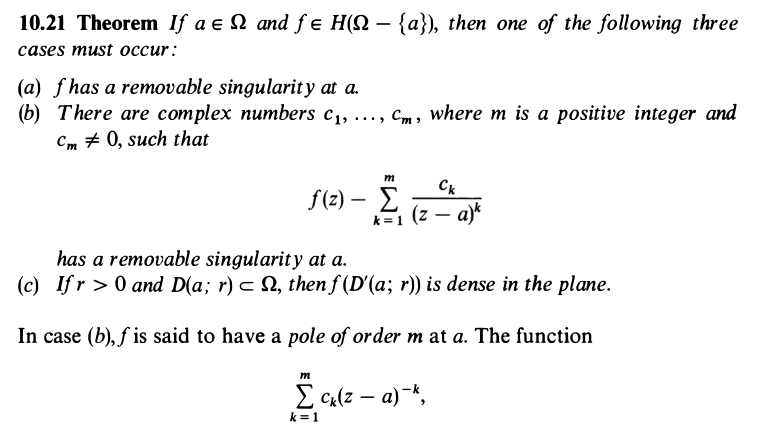
\includegraphics[width=\textwidth]{7-复分析脉络-2025040416.png}
% \caption{}
\label{}
\end{figure}

\begin{figure}[H]
\centering
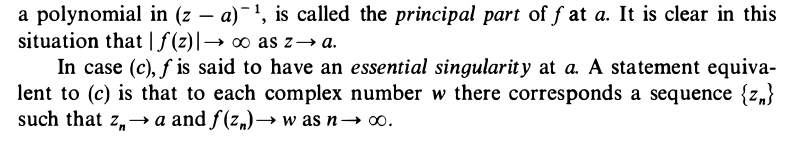
\includegraphics[width=\textwidth]{8-复分析脉络-2025040416.png}
% \caption{}
\label{}
\end{figure}

\begin{figure}[H]
\centering
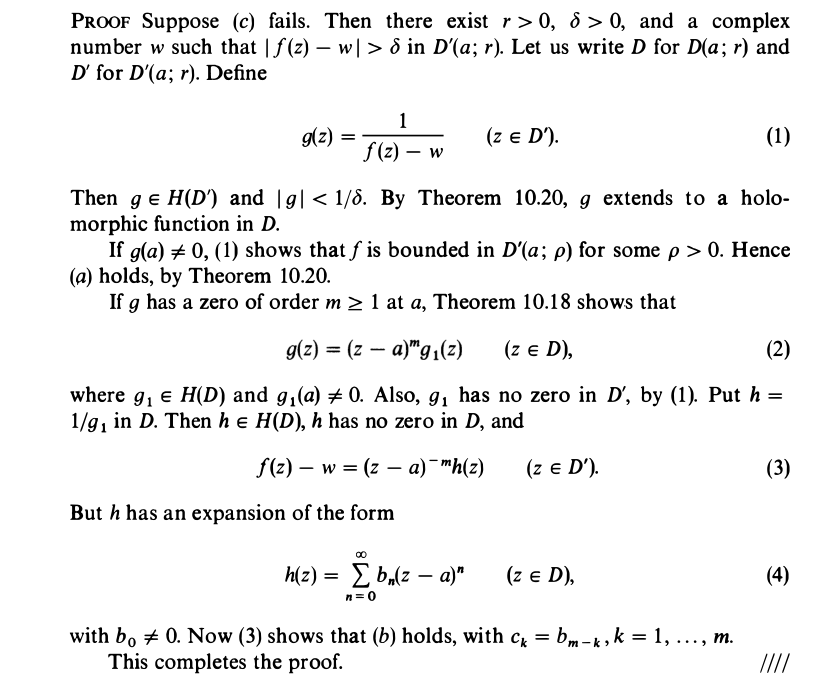
\includegraphics[width=\textwidth]{9-复分析脉络-2025040416.png}
% \caption{}
\label{}
\end{figure}

\begin{figure}[H]
\centering
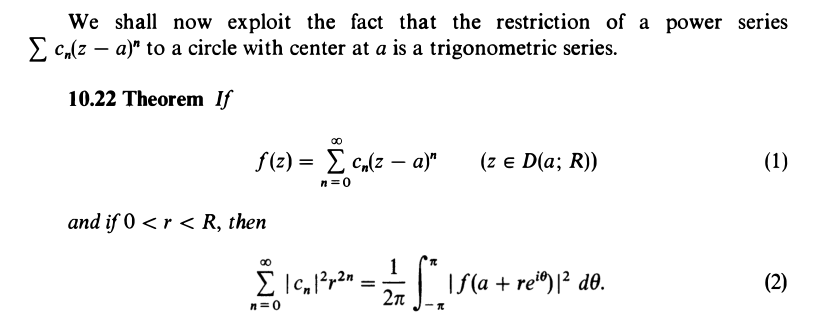
\includegraphics[width=\textwidth]{10-复分析脉络-2025040416.png}
% \caption{}
\label{}
\end{figure}

The proof is routine since
\[
\frac{1}{2\pi}\int_{-\pi}^{\pi} \underbrace{ \left\lvert  f(a+re^{ i\theta })   \right\rvert ^2}_{ \sum_{n=0}^{\infty} c_nr^{n}e^{ in\theta } }  \, d\theta = \frac{1}{2\pi}\sum_{n=0}^{\infty} \sum_{n'=0}^{\infty}  \int_{-\pi}^{\pi} c_n \overline{c_n}r^{2n}e^{ in\theta }e^{ -in'\theta } \, d\theta =\sum_{n=0}^{\infty} \lvert c_n \rvert ^2 r^{2n}
\]
Here are some consequences:

\begin{theorem}[Liouvill's theorem]
Every bounded entire function is constant.
\end{theorem}
\begin{proof}
Suppose $f$ entire, $f=\sum c_nz^{n}$ for all $z$, $\lvert f(z) \rvert<M$ for all $z$. Then
\[
\sum_{n=0}^{\infty} \lvert c_n \rvert ^2r^{2n}<M^2
\]
for all $r>0$, which is possible only if $c_n=0,\forall n$.
\end{proof}
\begin{figure}[H]
\centering
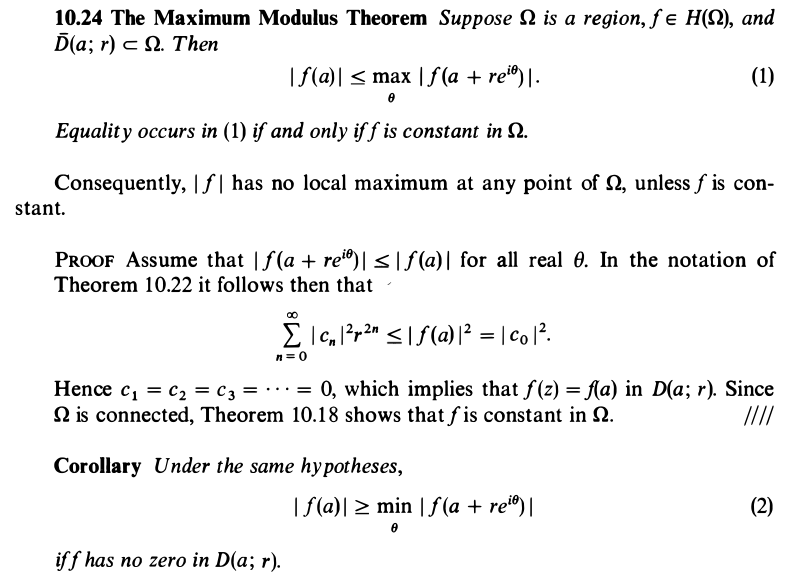
\includegraphics[width=\textwidth]{11-复分析脉络-2025040416.png}
% \caption{}
\label{}
\end{figure}

\subsubsection{The foundamental algebra theorem}

\begin{figure}[H]
\centering
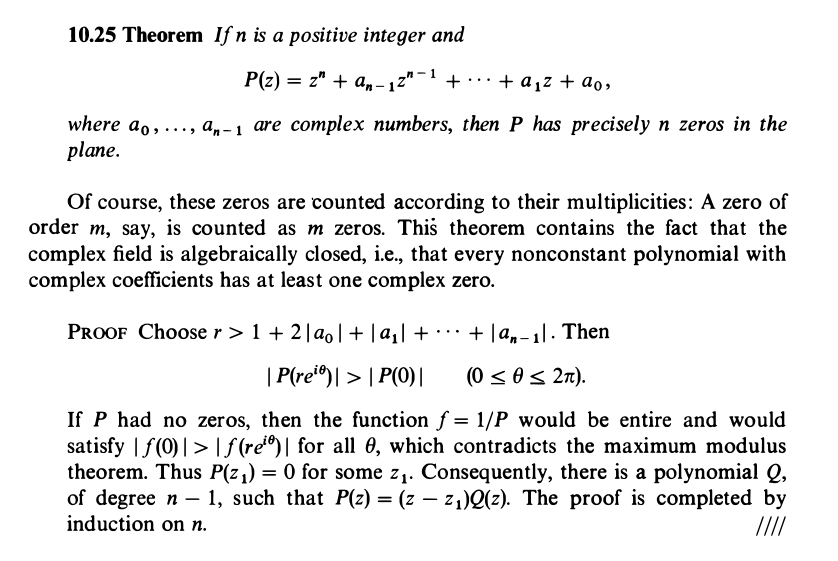
\includegraphics[width=\textwidth]{12-复分析脉络-2025040416.png}
% \caption{}
\label{}
\end{figure}

\subsubsection{Uniformly convergence}

\begin{figure}[H]
\centering
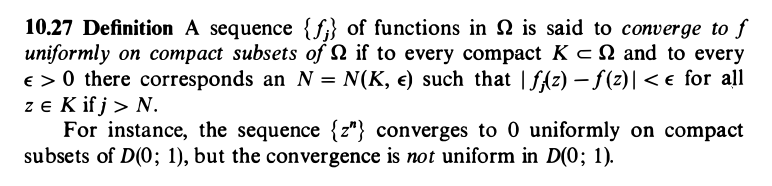
\includegraphics[width=\textwidth]{13-复分析脉络-2025040416.png}
% \caption{}
\label{}
\end{figure}

利用柯西积分公式可以给出如下定理的证明.

\begin{figure}[H]
\centering
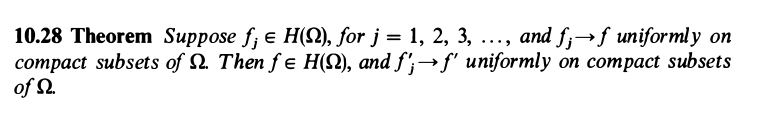
\includegraphics[width=\textwidth]{14-复分析脉络-2025040416.png}
% \caption{}
\label{}
\end{figure}

\subsubsection{Open mapping theorem}

\begin{figure}[H]
\centering
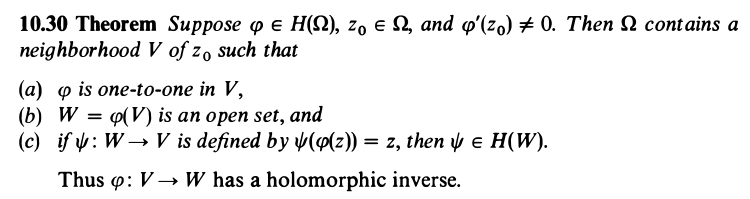
\includegraphics[width=\textwidth]{15-复分析脉络-2025040416.png}
% \caption{}
\label{}
\end{figure}

Every nonconstant holomorphic function in a region is \underline{locally} of the form $\pi_{m}\circ\varphi$ ($\pi_{m}:z\mapsto z^{m}$), except for an additive constant.

\begin{figure}[H]
\centering
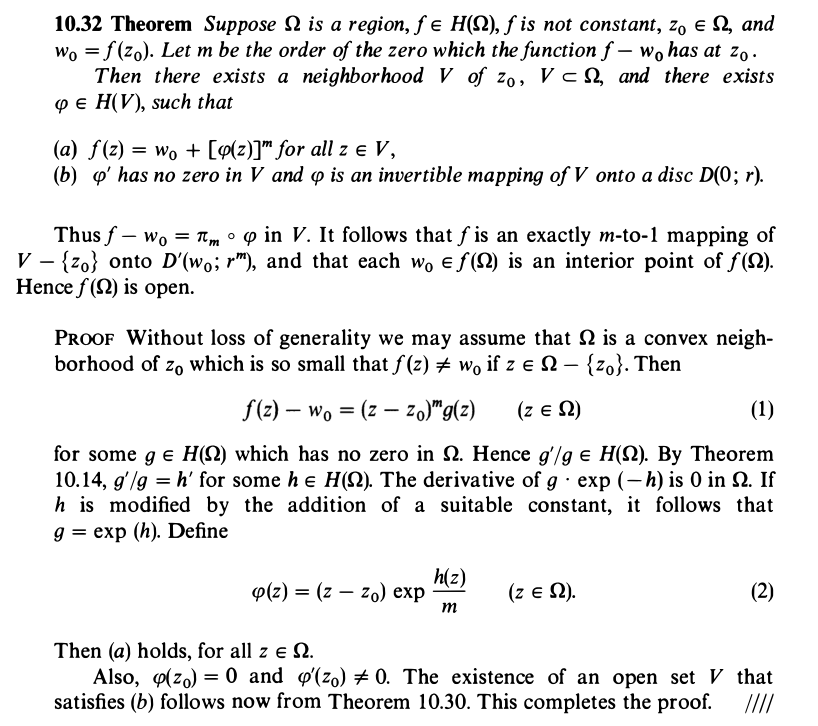
\includegraphics[width=\textwidth]{16-复分析脉络-2025040416.png}
% \caption{}
\label{}
\end{figure}

\begin{figure}[H]
\centering
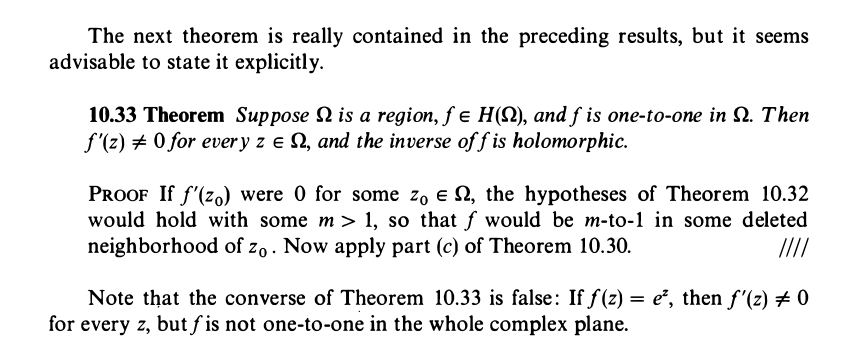
\includegraphics[width=\textwidth]{17-复分析脉络-2025040416.png}
% \caption{}
\label{}
\end{figure}

\subsubsection{Global Cauchy Theorem}

\paragraph{Definition of Chains and its properties}

\begin{figure}[H]
\centering
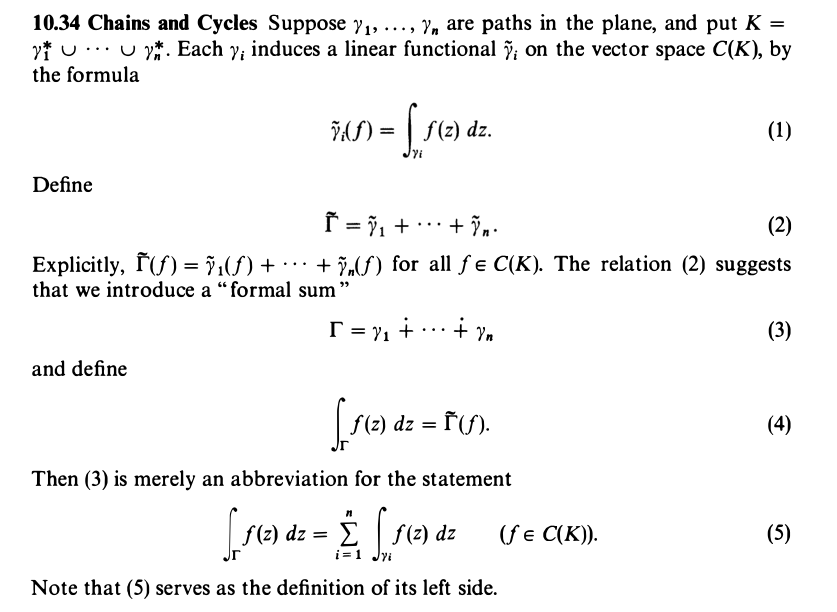
\includegraphics[width=\textwidth]{20-复分析脉络-2025040416.png}
% \caption{}
\label{}
\end{figure}
\begin{figure}[H]
\centering
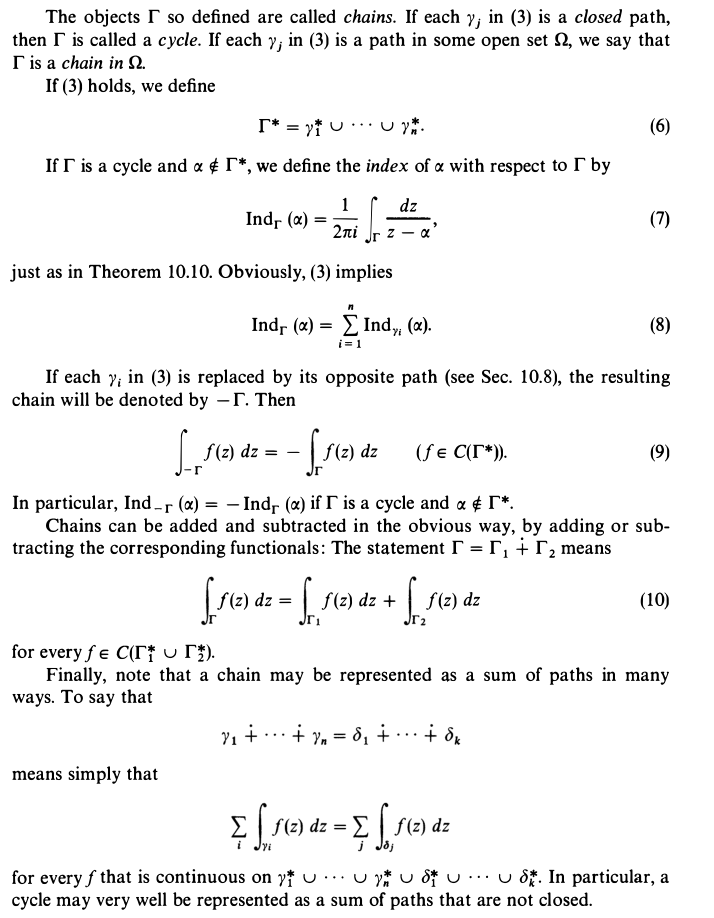
\includegraphics[width=\textwidth]{复分析脉络-2025040417.png}
% \caption{}
\label{}
\end{figure}

\paragraph{Cauchy's Theorem}

\begin{figure}[H]
\centering
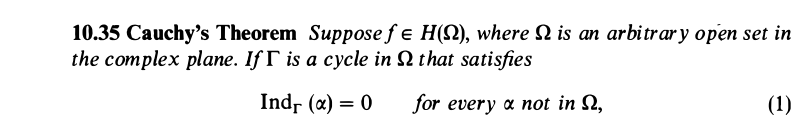
\includegraphics[width=\textwidth]{18-复分析脉络-2025040416.png}
% \caption{}
\label{}
\end{figure}

\begin{figure}[H]
\centering
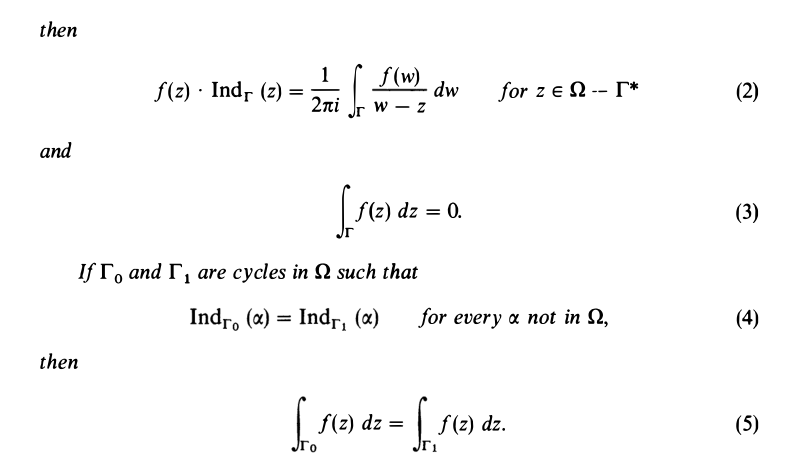
\includegraphics[width=\textwidth]{19-复分析脉络-2025040416.png}
% \caption{}
\label{}
\end{figure}

\subsubsection{Homotopy}

\begin{figure}[H]
\centering
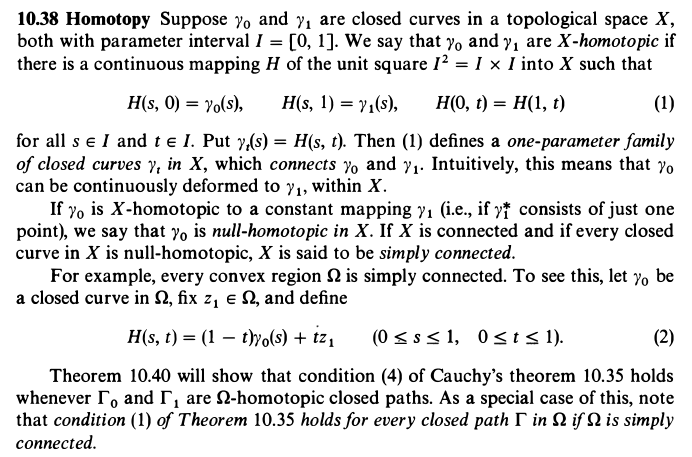
\includegraphics[width=\textwidth]{10-复分析脉络-2025040417.png}
% \caption{}
\label{}
\end{figure}
\begin{figure}[H]
\centering
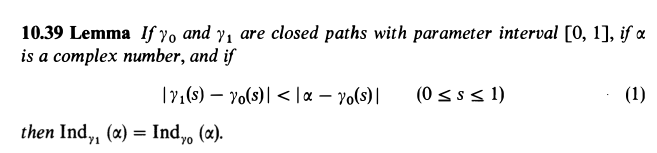
\includegraphics[width=\textwidth]{6-复分析脉络-2025040417.png}
% \caption{}
\label{}
\end{figure}
\begin{figure}[H]
\centering
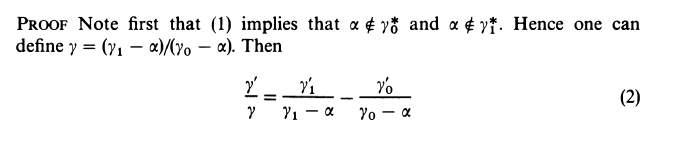
\includegraphics[width=\textwidth]{7-复分析脉络-2025040417.png}
% \caption{}
\label{}
\end{figure}
\begin{figure}[H]
\centering
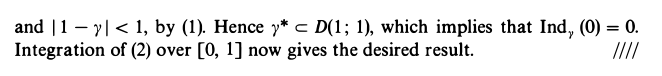
\includegraphics[width=\textwidth]{8-复分析脉络-2025040417.png}
% \caption{}
\label{}
\end{figure}
\begin{figure}[H]
\centering
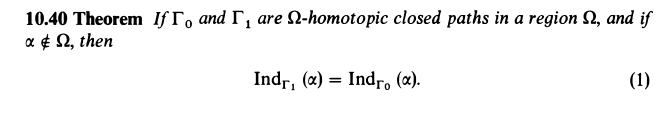
\includegraphics[width=\textwidth]{9-复分析脉络-2025040417.png}
% \caption{}
\label{}
\end{figure}

\subsubsection{Calculus of Residues}

\paragraph{Defintion of meromorphic function}

\begin{figure}[H]
\centering
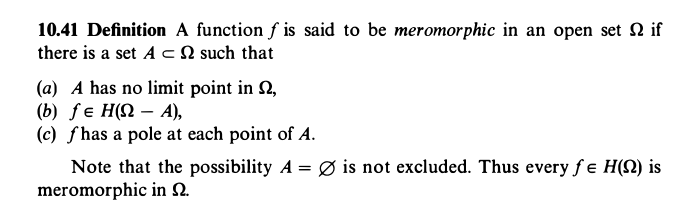
\includegraphics[width=\textwidth]{1-复分析脉络-2025040417.png}
% \caption{}
\label{}
\end{figure}

\paragraph{The residue theorem}

\begin{figure}[H]
\centering
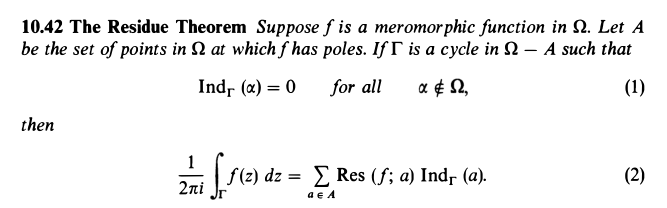
\includegraphics[width=\textwidth]{2-复分析脉络-2025040417.png}
% \caption{}
\label{}
\end{figure}

For $\Gamma=\gamma_1+\dots+\gamma_n$, $\mathrm{Ind}_{\Gamma}(\alpha)=\sum_{k=1}^{n}\mathrm{Ind}_{\gamma _k}(\alpha)$.

\paragraph{Two typical applications of the residue theorem}

The first one concerns zeros of holomorphic functions, the second is the evaluation of a certain integral.

\begin{figure}[H]
\centering
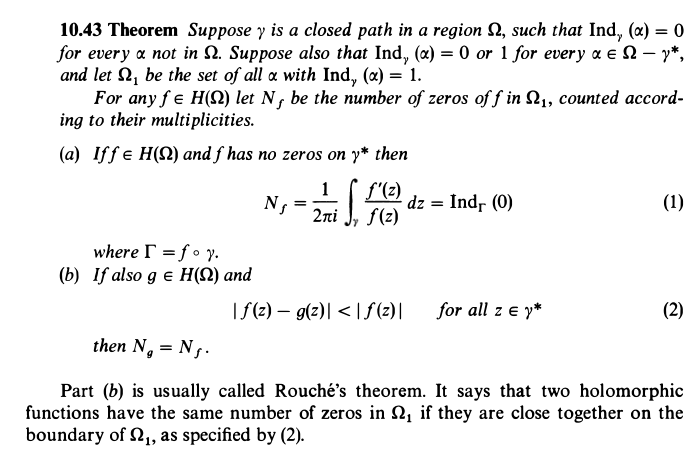
\includegraphics[width=\textwidth]{3-复分析脉络-2025040417.png}
% \caption{}
\label{}
\end{figure}

\begin{figure}[H]
\centering
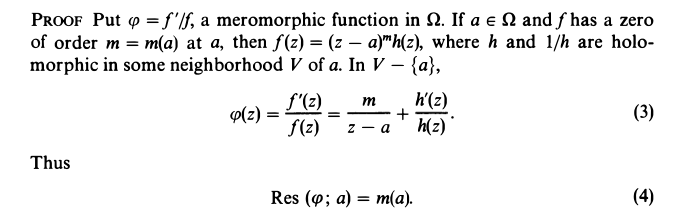
\includegraphics[width=\textwidth]{4-复分析脉络-2025040417.png}
% \caption{}
\label{}
\end{figure}

\begin{note}
$f'/f$ 在 $a$ 处的极点阶数恰恰等于其在 $a$ 处的留数.
\end{note}
\begin{figure}[H]
\centering
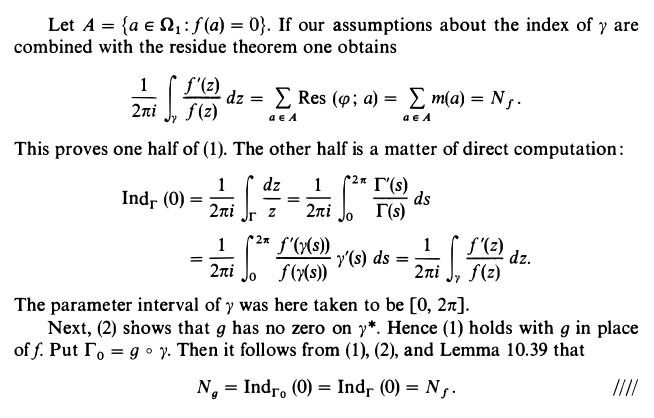
\includegraphics[width=\textwidth]{5-复分析脉络-2025040417.png}
% \caption{}
\label{}
\end{figure}
